\chapter{Układ sterowania i instrumentacji}
\label{cha:ch3_uklad_ster_i_instrumentacji}

Do odczytywania danych z obiektu i sterowania nim wykorzystano opisany w tym rozdziale układ sterowania i instrumentacji (\cref{fig:schemat_ukl_sterowania_instrumentacji}). W jego sercu znajduje się przemysłowy sterownik PLC, który odczytuje dane o położeniu kulki z dwóch czujników odległości oraz położenie kątowe wału wyjściowego motoreduktora z~enkodera przyrostowego kwadraturowego. Dodatkowo do sterownika podłączony został czujnik bazowania oraz przyciski: \texttt{START} (NO), \texttt{STOP} (NC). Na wyjścia sterownika podłączony został mostek H kontrolujący silnik oraz dioda świecąca sygnalizacyjna.

\begin{figure}[H]
    \centering
    \includesvg[width=\textwidth,svgpath=./vector_graphics/]{uklad_sterowania_i_instrumentacji}
    % 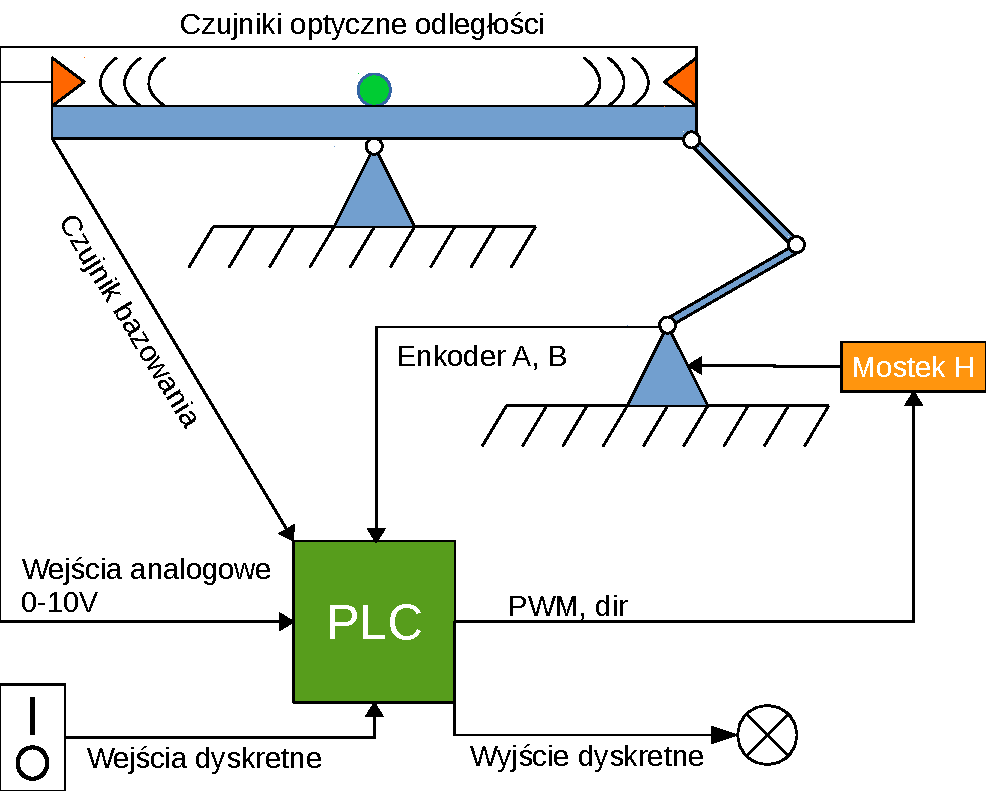
\includegraphics[width=0.7\textwidth]{schemat_ukladu3}
    \caption{Schemat układu sterowania i instrumentacji wraz z zaznaczonymi połączeniami.}
    \label{fig:schemat_ukl_sterowania_instrumentacji}
\end{figure}

%%%%%%%%
\section{Sterownik PLC}
\label{sec:ch3_PLC}

Wykorzystany w pracy sterownik PLC to \textsc{Simatic S7-1211C DC/DC/DC} firmy Siemens. Działa on na napięciu stałym \SI{24}{V}, posiada 6 wejść dyskretnych \SI{24}{V}, 4 tranzystorowe wyjścia dyskretne \SI{24}{V} i 2 napięciowe wejścia analogowe \SIrange{0}{10}{V}.

W celu ułatwienia komunikacji między sterownikiem i elektroniką opartą o logikę \SI{5}{V} (więcej w~rozdziale \ref{sec:ch3_systemy_napiec}), został on rozszerzony o dodatkową płytkę sygnałową SB 1223 działającą na logice \SI{5}{V}; dodaje ona po 2 wejścia i~wyjścia dyskretne \SI{5}{V}. Sterownik z już zamontowaną płytką przedstawiono na \cref{fig:sterownik_plytka_sygn}.

Podstawowe parametry sterownika oraz płytki sygnałowej zostały zebrane w tabeli \ref{tab:parametry_PLC_SB}:

\begin{table}[H]
    \centering
    \begin{threeparttable}
        \caption{Podstawowe parametry sterownika PLC Siemens S7-1211C i płytki sygnałowej Siemens SB 1223\tnote{a}.}
        \label{tab:parametry_PLC_SB}
        
        \begin{tabular}{p{4.5cm} | l | l}
            \toprule
            Nazwa & Siemens S7-1211C & Siemens SB 1223 \\
            \midrule
            Napięcie zasilania & \SI{24}{V} DC & \SI{5}{V} DC \\
            \midrule
            Liczba wejść cyfrowych & 6 & 2 \\
            Liczba wyjść cyfrowych & 4 & 2 \\
            Liczba wejść analogowych & 2 & 0 \\
            Liczba wyjść analogowych & 0 & 0 \\
            Typ wejść cyfrowych & \textit{sink-source} & \textit{source} \\
            Typ wyjść cyfrowych & MOSFET \textit{source} & MOSFET \textit{sink-source} \\
            Typ wejść analogowych & Napięciowe \SIrange{0}{10}{V} & n.d. \\
            \midrule
            Szybkie liczniki & Do 6 z częstotliwością \SI{100}{kHz}\tnote{b} & Do 2 z częstotliwością \SI{200}{kHz}\tnote{c} \\
            Wyjścia impulsowe & Do 4 z częstotliwością \SI{100}{kHz} & Do 2 z częstotliwością \SI{200}{kHz} \\
            \midrule
            Pamięć robocza & \SI{30}{kB} & n.d. \\
            Pamięć ładowania & \SI{1}{MB} & n.d. \\
            Pamięć trwała & \SI{10}{kB} & n.d. \\
            \midrule
            Czas wykonywania instrukcji boolowskich & \SI{0,08}{\micro\second}/instrukcję & n.d. \\
            Czas wykonywania operacji na typie WORD & \SI{1,7}{\micro\second}/instrukcję & n.d. \\
            Czas wykonywania operacji na typie REAL & \SI{2,3}{\micro\second}/instrukcję & n.d. \\
            \bottomrule
        \end{tabular}
        
        \begin{tablenotes}
            \footnotesize
            \item[a] opracowanie własne na podstawie \cite{S7MANUAL},
            \item[b] w trybie kwadraturowym wykorzystywane są dwa wejścia, a~maksymalna częstotliwość wynosi \SI{80}{kHz},
            \item[c] w trybie kwadraturowym wykorzystywane są dwa wejścia, a~maksymalna częstotliwość wynosi \SI{160}{kHz}.
        \end{tablenotes}
    \end{threeparttable}
\end{table}

\begin{figure}[h]
    \centering
    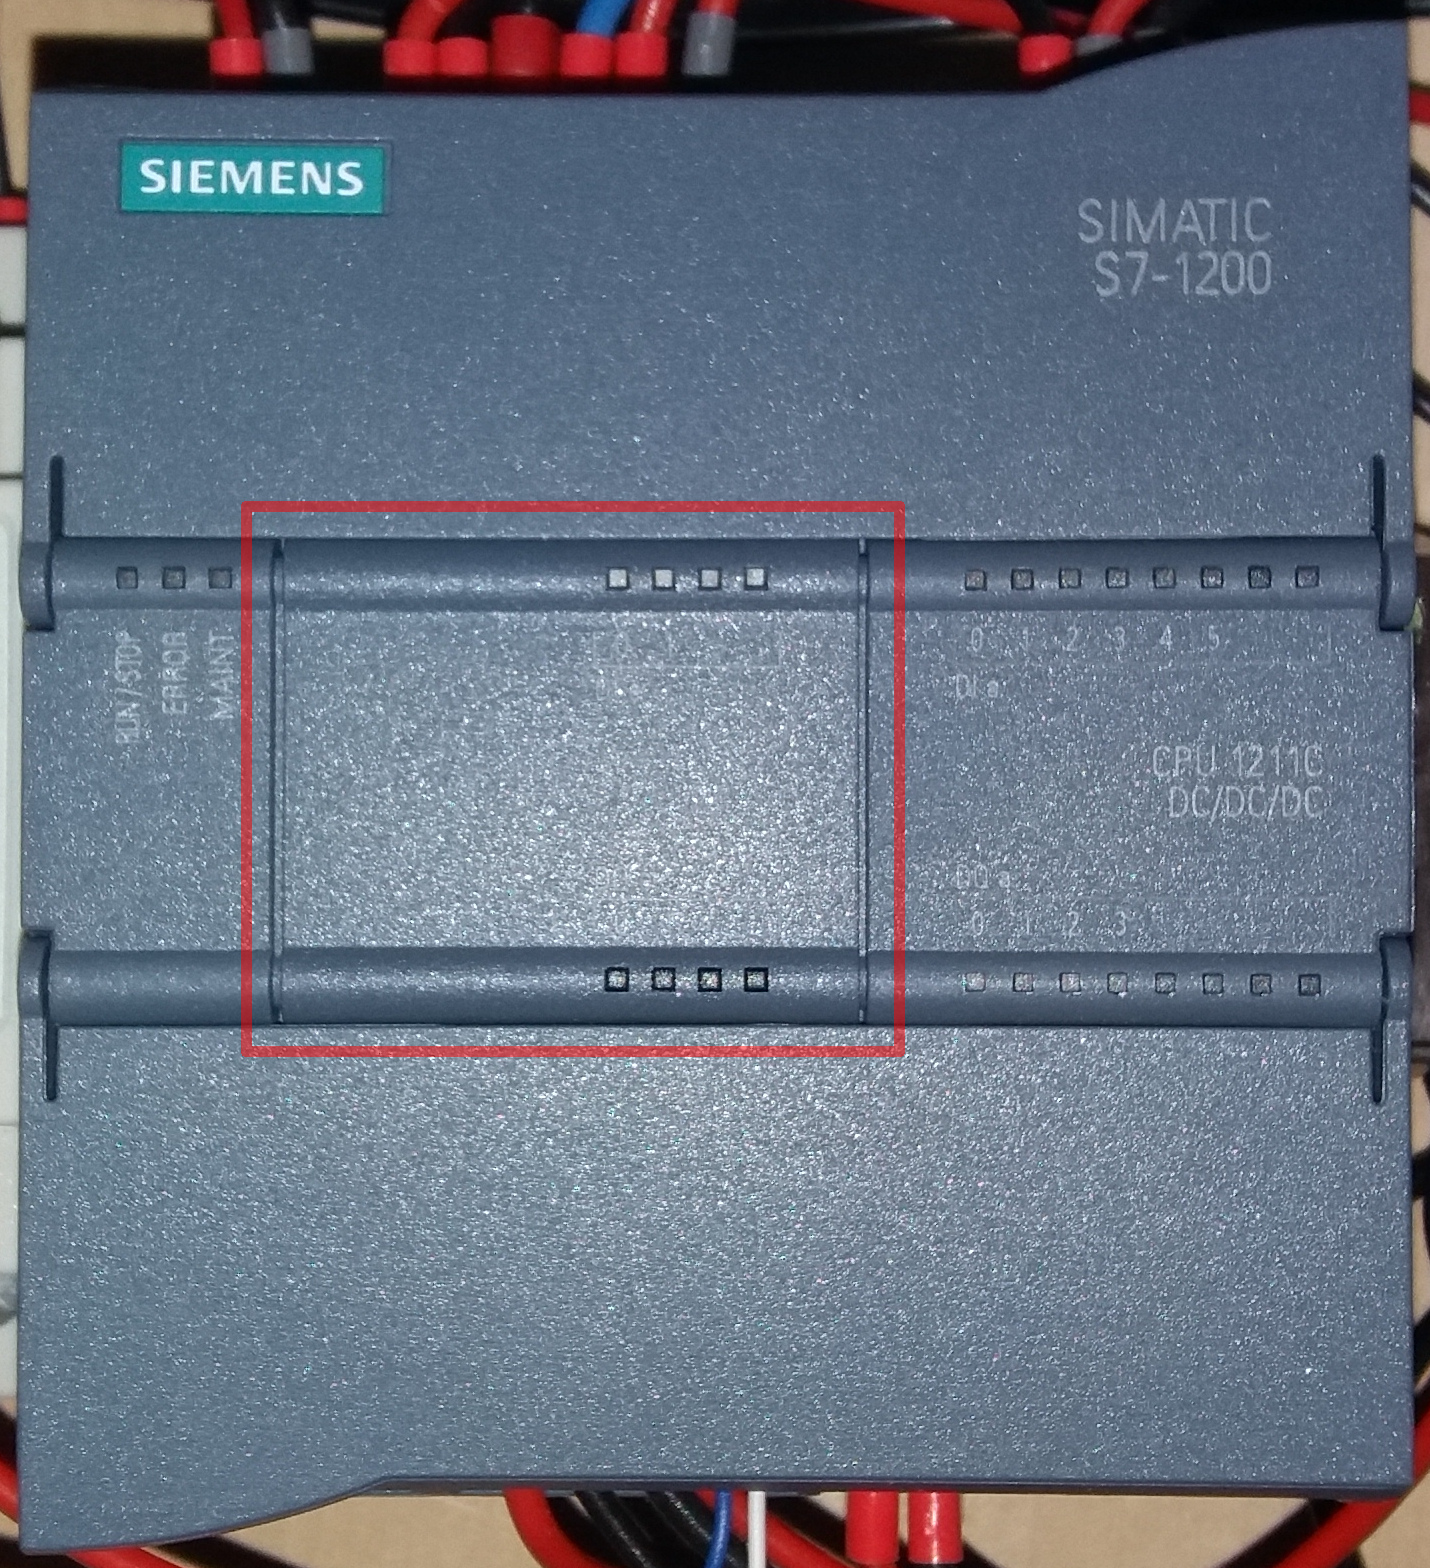
\includegraphics[width=0.5\textwidth]{s71200_sb1223}
    \caption{Zdjęcie użytego sterownika z zaznaczoną płytką sygnałową.}
    \label{fig:sterownik_plytka_sygn}
\end{figure}

%%%%%%%%
\section{Silnik z reduktorem i enkoderem}
\label{sec:ch3_uklad_napedowy}

Jak już zasygnalizowano w rozdziale \ref{sec:ch2_przeniesienie_napedu}, w pracy użyto silnik prądu stałego (komutatorowy, z~magnesami trwałymi). Silnik sprzężony jest z~zębatą przekładnią redukcyjną o przełożeniu \num{18,75}:\num{1} (całość nazywana jest motoreduktorem). Na wale silnika zamocowany jest enkoder inkrementalny kwadraturowy o~64 impulsach na obrót wału, co daje 1200 impulsów za przekładnią. Zdjęcie silnika przedstawiono na \cref{fig:silnik}.

Wybrany silnik stanowi dobry kompromis między złożonością, wydajnością i ceną. Dyskusja na temat możliwości zastosowania innych typów napędów została przeprowadzona w dodatku \ref{appA_warianty_zespolu_napedowego}.

\begin{figure}[h]
    \centering
    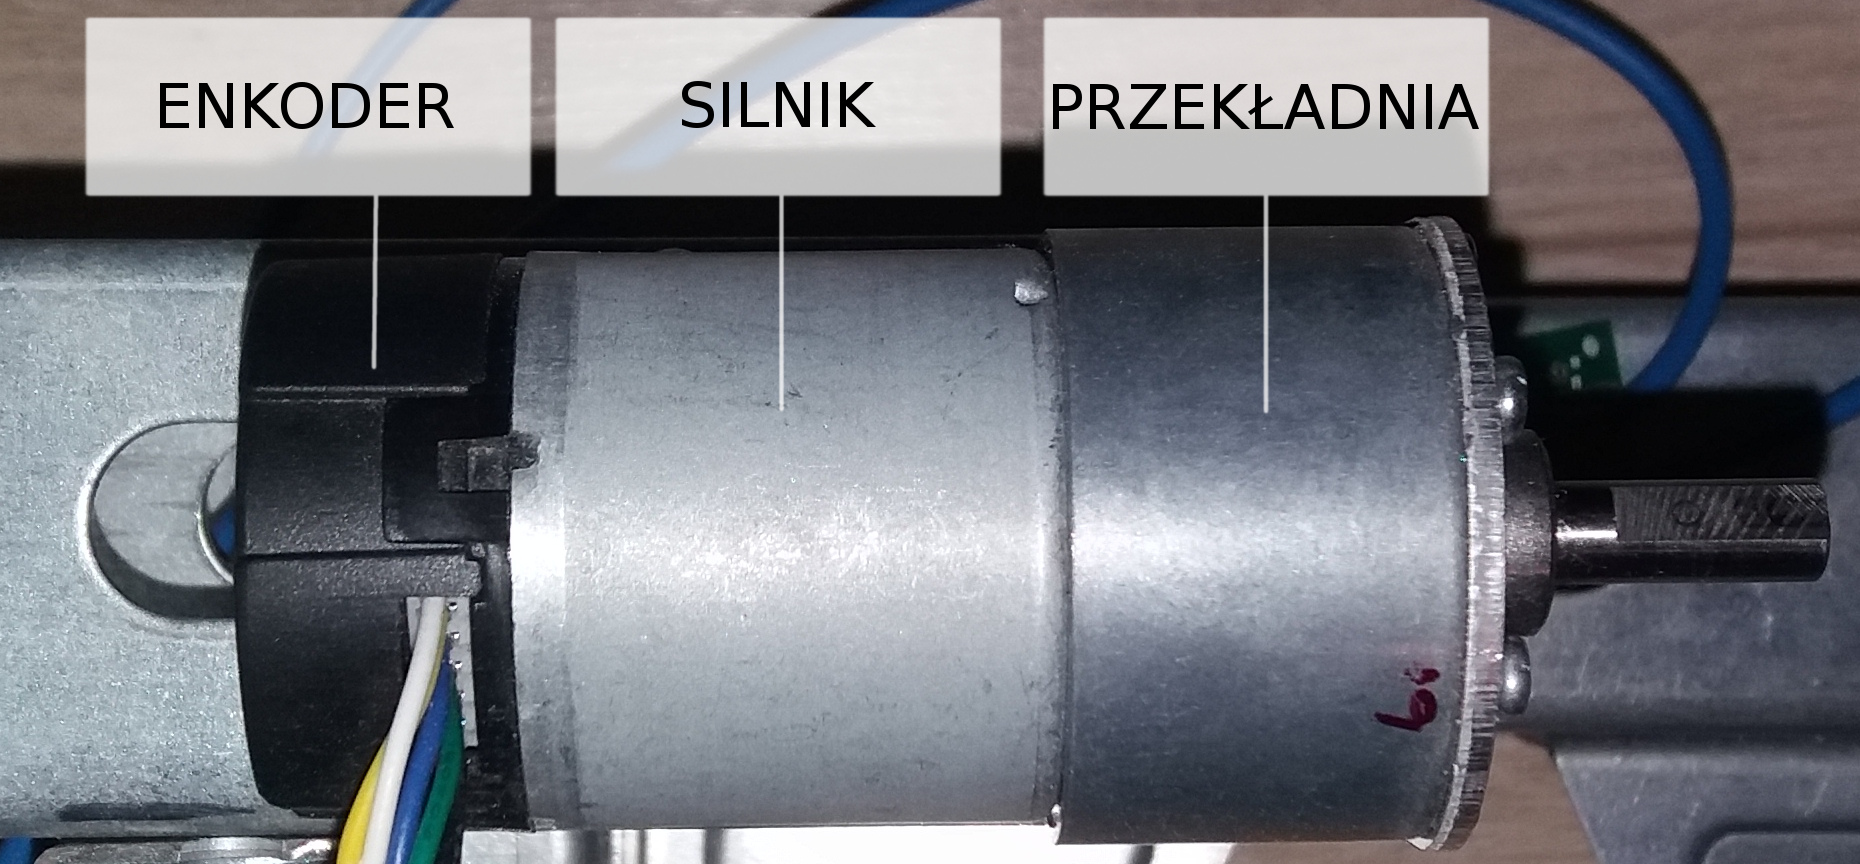
\includegraphics[width=0.55\textwidth]{silnik}
    \caption{Zdjęcie silnika w rzucie od góry z zaznaczoną przekładnią oraz enkoderem.}
    \label{fig:silnik}
\end{figure}

Producent silnika nie dostarcza doń pełnej dokumentacji, a jedynie wartości kilku wybranych parametrów. Wymusiło to analityczne lub eksperymentalne wyznaczenie pozostałych wymaganych do zamodelowania silnika parametrów. Wszystkie podane parametry zostały przedstawione w tabeli \ref{tab:parametry_silnika} poniżej.

\begin{table}[H]
    \centering
    \begin{threeparttable}
        \caption{Parametry podane przez producenta silnika\tnote{a}, enkodera i przekładni\tnote{b}.}
        \label{tab:parametry_silnika}
        
        \begin{tabularx}{0.9\textwidth}{l | l}
            \toprule
            Parametr & Wartość \\
            \midrule
            Średnica & \SI{37}{\milli\meter} \\
            Długość & \SI{68}{\milli\meter} \\
            Masa & \SI{215}{g} \\
            Średnica wału & \SI{6}{\milli\meter} \\
            \midrule
            Przełożenie przekładni & \num{18,75}:\num{1} \\
            \midrule
            Napięcie znamionowe & \SI{12}{\volt} \\
            Prędkość biegu jałowego & \SI{52,36}{\radian\per\second} \\
            Prąd biegu jałowego & \SI{300}{\milli\ampere} \\
            Prąd zatrzymania silnika & \SI{5000}{\milli\ampere} \\
            Moment zatrzymania silnika & \SI{0,59}{\newton\meter} \\
            \midrule
            Typ enkodera & Kwadraturowy, inkrementalny, bez pamięci \\
            Liczba impulsów na obrót za przekładnią & \num{1200} (tryb kwadraturowy) \\
            \bottomrule
        \end{tabularx}
        
        \begin{tablenotes}
            \footnotesize
            \item[a] niektóre parametry silnika w rzeczywistości mają inne wartości, zob. rozdział \ref{sec:ch5_identyfikacja_parametrow_silnika},
            \item[b] opracowanie własne na podstawie \cite{SILNIK_MANUAL}.
        \end{tablenotes}
    \end{threeparttable}
\end{table}

Parametry niewymienione w tabeli \ref{tab:parametry_silnika}, takie jak rezystancja silnika, stała silnika, moment bezwładności wału czy współczynniki tarcia suchego i wiskotycznego, nie zostały podane przez producenta, dlatego przeprowadzono ich identyfikację opisaną w rozdziale \ref{sec:ch5_identyfikacja_parametrow_silnika}.

Silnik sterowany jest przez PLC za pomocą układu scalonego mostka H z~tranzystorami MOSFET (Pololu BD65496MUV). Został on dobrany tak, by spełniać wymagania elektryczne silnika przy pracy znamionowej. Sterowany jest sygnałem PWM o częstotliwości \SI{20}{\kilo\hertz}. Dodatkowym sygnałem jest binarny sygnał kierunku obrotu silnika. Najistotniejsze parametry wybranego mostka H przedstawiono w~tabeli \ref{tab:parametry_mostka_H}.

\begin{table}[H]
    \centering
    \begin{threeparttable}
        \caption{Najważniejsze parametry mostka H\tnote{a}.}
        \label{tab:parametry_mostka_H}
        
        \begin{tabular}{l | l}
            \toprule
            Parametr & Wartość \\
            \midrule
            Napięcie pracy silnika & \SIrange{2}{16}{\volt} \\
            Maksymalny prąd ciągły silnika & \SI{1,2}{\ampere} \\
            Maksymalny prąd chwilowy silnika & \SI{5}{\ampere} \\
            Maksymalna częstotliwość PWM & \SI{500}{\kilo\hertz} \\
            Napięcie zasilania części logicznej & \SIrange{2,5}{5,5}{\volt} \\
            Napięcie sygnałów logicznych & Napięcie zasilania \SI{+-0,3}{\volt} \\
            \bottomrule
        \end{tabular}
        
        \begin{tablenotes}
            \footnotesize
            \item[a] opracowanie własne na podstawie \cite{MOSTEK_H_MANUAL}.
        \end{tablenotes}
    \end{threeparttable}
\end{table}

Wszystkie wymagane połączenia elektryczne wykonano na uniwersalnej płytce PCB, na której umieszczono niezbędne złącza i listwy zaciskowe. Do tej samej płytki wlutowano również wspomniany mostek H, którego zdjęcie przedstawiono na \cref{fig:zdjecie_mostka_H}, a opis złącz w tabeli \ref{tab:zlacza_mostka_H}. Zdjęcie płytki PCB przedstawiono na \cref{fig:mostek_H_PCB}.

\begin{figure}[h]
    \centering
    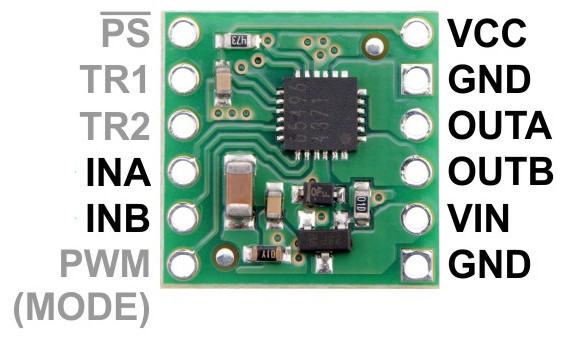
\includegraphics[width=0.4\textwidth]{mostek_H}
    \caption{Zdjęcie układu mostka H (Pololu BD65496MUV). Źródło: \url{https://www.pololu.com/product/2960}.}
    \label{fig:zdjecie_mostka_H}
\end{figure}

% TODO: schemat ideowy modułu (ze źródła)

\begin{table}[H]
    \centering
    \begin{threeparttable}
        \caption{Opis złącz mostka H\tnote{a}.}
        \label{tab:zlacza_mostka_H}
        
        \begin{tabularx}{0.67\textwidth}{l | l}
            \toprule
            Złącze & Opis \\
            \midrule
            \texttt{VCC} & Zasilanie układu \\
            \texttt{VIN} & Zasilanie silnika \\
            \texttt{GND} & Masa \\
            \texttt{OUTA}, \texttt{OUTB} & Wyjścia zasilania silnika \\
            \texttt{INA}, \texttt{INB} & Wejścia sygnałów sterujących \\
            \texttt{PWM (MODE)} & Przełączanie między trybem \texttt{IN/IN} a~\texttt{EN/IN}\tnote{b} \\
            \texttt{PS} & Oszczędzanie energii \\
            \texttt{TR1}, \texttt{TR2} & Kontrola maksymalnej częstotliwości \\
            \bottomrule
        \end{tabularx}
        
        \begin{tablenotes}
            \footnotesize
            \item[a] opracowanie własne na podstawie \cite{MOSTEK_H_MANUAL},
            \item[b] układ umożliwia sterowanie silnikiem w trybie \texttt{IN/IN} oraz \texttt{EN/IN}; ten pierwszy przekazuje sygnał wysoki ze złącza \texttt{INA} na \texttt{OUTA} i \texttt{INB} na \texttt{OUTB} (za wyjątkiem sytuacji dwóch stanów wysokich), natomiast ten drugi pozwala użyć sygnału PWM (\texttt{INA}) oraz sygnału kierunku obrotu (\texttt{INB}).
        \end{tablenotes}
    \end{threeparttable}
\end{table}

W układzie nie zastosowano czujnika położenia wału, do którego przymocowana jest belka; zamiast tego wykorzystano zależność geometryczną pomiędzy obrotem wału motoreduktora a obrotem belki. W przypadku niewielkich odchyleń kąt belki $\theta$ powinien być w przybliżeniu liniowo związany z kątem obrotu wału motoreduktora $\alpha$~w~następujący sposób:

\begin{equation}\label{eq:uproszczona_zaleznosc_kata_belki}
    \theta = \frac{d_L}{d_k} \alpha
\end{equation}
gdzie: $d_L$ to odległość końca belki od osi obrotu, a $d_k$ to długość korby. Zależność \eqref{eq:uproszczona_zaleznosc_kata_belki} wynika z~założenia, że punkty zaczepu korbowodu przebędą taką samą drogę łukową, a zatem $\theta d_k = \alpha d_L$.

Niestety, równanie \eqref{eq:uproszczona_zaleznosc_kata_belki} jest poprawne tylko w niewielkich odchyleniach belki od poziomu oraz gdy linia łącząca punkt zaczepu mechanizmu korbowego i oś obrotu belki jest równoległa do korby. Faktyczna zależność $\theta(\alpha)$ została zidentyfikowana za pomocą modelu symulacyjnego (rozdział \ref{sec:ch4_zaleznosc_kata_silnika_i_kata_belki}).

\begin{figure}[H]
    \centering
    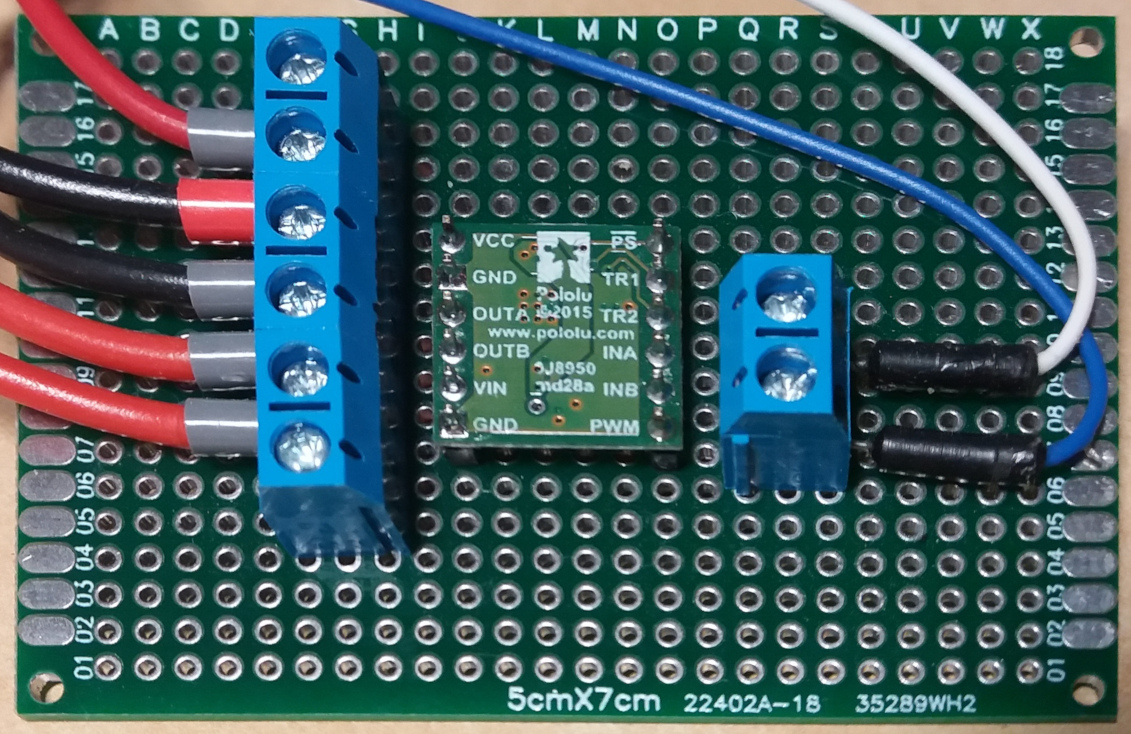
\includegraphics[width=0.6\textwidth]{mostek_H_PCB}
    \caption{Zdjęcie płytki PCB z zamontowanym układem mostka H (Pololu BD65496MUV).}
    \label{fig:mostek_H_PCB}
\end{figure}

%%%%%%%%
\section{Czujniki odległości}
\label{sec:ch3_czujniki_odleglosci}

Do pomiaru położenia kulki wykorzystano parę analogowych czujników Sharp GP2Y0A41SK0F (\cref{fig:czujnik_sharp}). Każdy z czujników składa się z nadajnika światła podczerwonego i odbiornika; obliczanie pozycji obiektu odbywa się na zasadzie triangulacji. Podstawowe parametry czujników opisano w~tabeli~\ref{tab:parametry_czujnikow_Sharp}.

\begin{figure}[h]
    \centering
    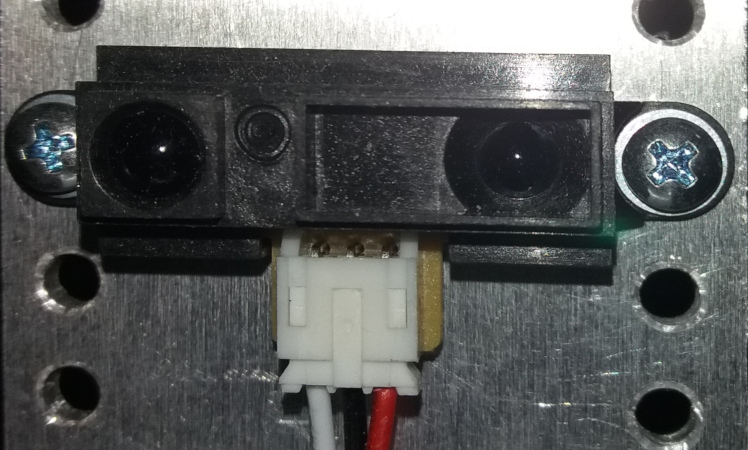
\includegraphics[width=0.5\textwidth]{czujnik}
    \caption{Zdjęcie czujnika Sharp GP2Y0A41SK0F.}
    \label{fig:czujnik_sharp}
\end{figure}

Czujniki optyczne pracujące w podczerwieni nie są jedynymi sensorami, które można zastosować do badania położenia kulki w układach typu kulka i belka. Alternatywne sposoby zostały omówione w~dodatku \ref{appB_alternatywne_czujniki_pozycji_kulki}.

\begin{table}[h]
    \centering
    \begin{threeparttable}
        \caption{Podstawowe parametry czujników pozycji kulki\tnote{a}.}
        \label{tab:parametry_czujnikow_Sharp}
        
        \begin{tabularx}{0.75\textwidth}{l | l}
            \toprule
            Parametr & Wartość \\
            \midrule
            Napięcie zasilania & \SIrange{4,5}{5,5}{\volt} \\
            Zakres pomiarowy & \SIrange{4}{30}{\centi\meter} \\
            Typ sygnału wyjściowego & Analogowy napięciowy około \SIrange{0,25}{3,1}{\volt} \\
            \bottomrule
        \end{tabularx}
        
        \begin{tablenotes}
            \footnotesize
            \item[a] opracowanie własne na podstawie \cite{SHARP_MANUAL}.
        \end{tablenotes}
    \end{threeparttable}
\end{table}

Czujniki zostały zamontowane na wspornikach umożliwiających regulację wysokości oraz pochylenia względem belki (zob. rozdział \ref{sec:ch2_belka}). Odległość między czujnikami to \SI{40}{\centi\meter} (powyżej górnej granicy zakresu pomiarowego), a ich wysokość nad belką to \SI{4}{\centi\meter}. W dalszej części pracy, czujnik zamontowany dalej od punktu zaczepu korbowodu nazywany jest ,,lewy'', natomiast czujnik zamontowany bliżej tego punktu --- ,,prawy''.

Charakterystyka każdego z czujników jest nieróżnowartościowa i mocno nieliniowa (zob. \cref{fig:charakterystyka_czujnikow}). Dobrą aproksymację charakterystyki można otrzymać (po odcięciu wartości poniżej \SI{3}{\centi\meter}) za pomocą funkcji postaci $y =\nobreak a x ^ b + c$ (zob. tabela \ref{tab:aproksymacja_czujnikow}), gdzie $x$ to wartość pomiaru z przetwornika, a $y$ to odległość do przeszkody.

Sposób zebrania charakterystyk czujników oraz wykonana aproksymacja zostały opisane w rozdziale~\ref{sec:ch5_identyfikacja_charakterystyk_czujnikow}.

\begin{figure}[h]
    \centering
    \includesvg[width=\textwidth,svgpath=./vector_graphics/]{charakterystyka_czujnikow}
    \caption{Charakterystyka czujników odległości.}
    \label{fig:charakterystyka_czujnikow}
\end{figure}

Z powodu dużej złożoności obliczeniowej liczenia potęg niecałkowitych zrezygnowano z implementacji takich aproksymacji w sterowniku PLC. Wobec tych utrudnień zastosowano inne rozwiązanie w~celu obliczenia pozycji kulki: aproksymację liniową pomiędzy punktami charakterystyki. W tym celu wprowadzono punkty charakterystyki każdego z czujników (pary: wartość z przetwornika ADC, odległość do kulki) do dwóch tablic w sterowniku PLC.

Oba czujniki są równoodległe ($x_d = \SI{20}{\centi\meter}$) od środka belki, co oznacza, że aby uzyskać wychylenie środka kulki od środka belki, należy transformować układy odniesienia czujników, co ilustruje \cref{fig:polozenie_kulki}. Mając dwie odległości $d_l$ oraz $d_r$ od czujników do kulki, pozycję kulki $d_b$ oblicza się w~następujący sposób:
\begin{equation}\label{eq:pozycja_kulki}
d_b = \frac{d_l + 2\cdot d_c - d_r}{2} - d_c = \frac{d_l - d_r}{2}
\end{equation}

\begin{figure}[H]
    \centering
    \includesvg[width=0.5\textwidth,svgpath=./vector_graphics/]{pozycja_kulki}
    \caption{Położenie kulki względem środka belki i czujników.}
    \label{fig:polozenie_kulki}
\end{figure}


%%%%%%%%
\section{Czujnik bazowania}
\label{sec:ch3_czujnik_bazowania}

Z powodu wykorzystania enkodera inkrementalnego, po każdym uruchomieniu urządzenia konieczne jest przeprowadzenie procedury bazowania (zob. rozdział \ref{sec:ch7_bazowanie}) w celu określenia dokładnej pozycji kątowej wału motoreduktora, a co za tym idzie: pozycji kątowej belki.

Do wykrycia pozycji bazowania wykorzystano transoptor szczelinowy TCST1103 firmy Vishay Semiconductors połączony w układzie przedstawionym na \cref{fig:uklad_transoptora}, natomiast podstawowe parametry transoptora zostały opisane w tabeli \ref{tab:parametry_transoptora}.

% TODO: dobrze byłoby dodać szeregowo diody prostownicze bądź impulsowe o napięciu zaporowym ponad 24V, co uchroniłoby układ przed omyłkową zmianą biegunów zasilania
\begin{figure}[H]
    \centering
    \includesvg[width=0.8\textwidth,svgpath=./vector_graphics/]{uklad_transoptora}
    % 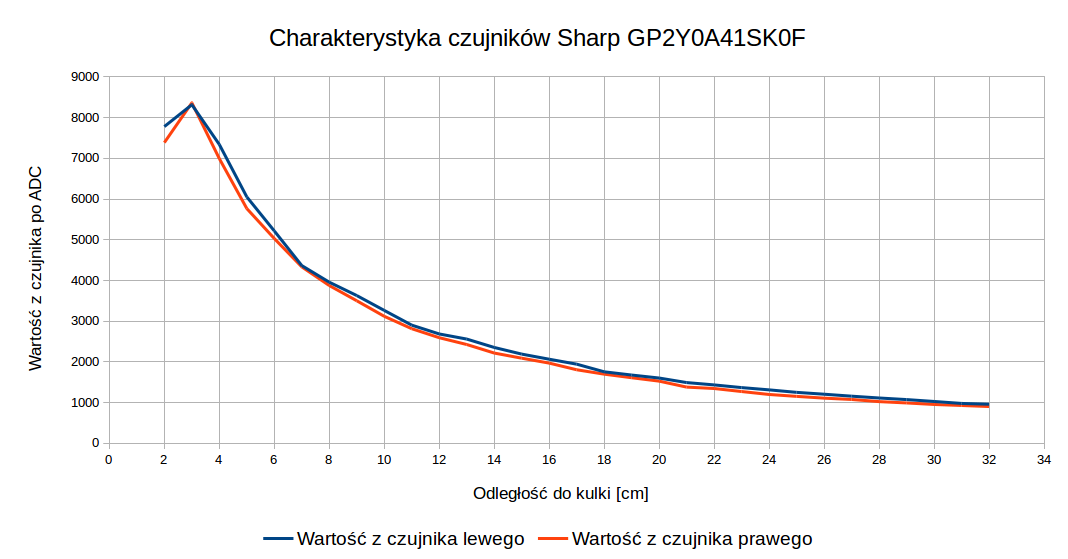
\includegraphics[width=1\textwidth]{sensor_characteristics}
    \caption{Schemat podłączenia układu transoptora.}
    \label{fig:uklad_transoptora}
\end{figure}

\begin{table}[h]
    \centering
    \begin{threeparttable}
        \caption{Podstawowe parametry transoptora szczelinowego\tnote{a}.}
        \label{tab:parametry_transoptora}
        
        \begin{tabularx}{0.6\textwidth}{l | l}
            \toprule
            Parametr & Wartość \\
            \midrule
            Szerokość szczeliny & \SI{3}{\milli\meter} \\
            Maks. prąd przewodzenia diody & \SI{60}{\milli\ampere} \\
            Maks. napięcie kolektor-emiter & \SI{70}{\volt} \\
            Współczynnik przekładni prądowej & \num{0,2} \\
            \bottomrule
        \end{tabularx}
        
        \begin{tablenotes}
            \footnotesize
            \item[a] opracowanie własne na podstawie \cite{TRANSOPTOR_MANUAL}.
        \end{tablenotes}
    \end{threeparttable}
\end{table}

Układ z \cref{fig:uklad_transoptora} przylutowano do płytki uniwersalnej (\cref{fig:czujnik_bazowania_PCB}). Elementy \texttt{J1} oraz \texttt{J2} reprezentują złącza zaciskowe, za pomocą których zrealizowano połączenia elektryczne z zasilaniem oraz sterownikiem PLC.

\begin{figure}[h]
    \centering
    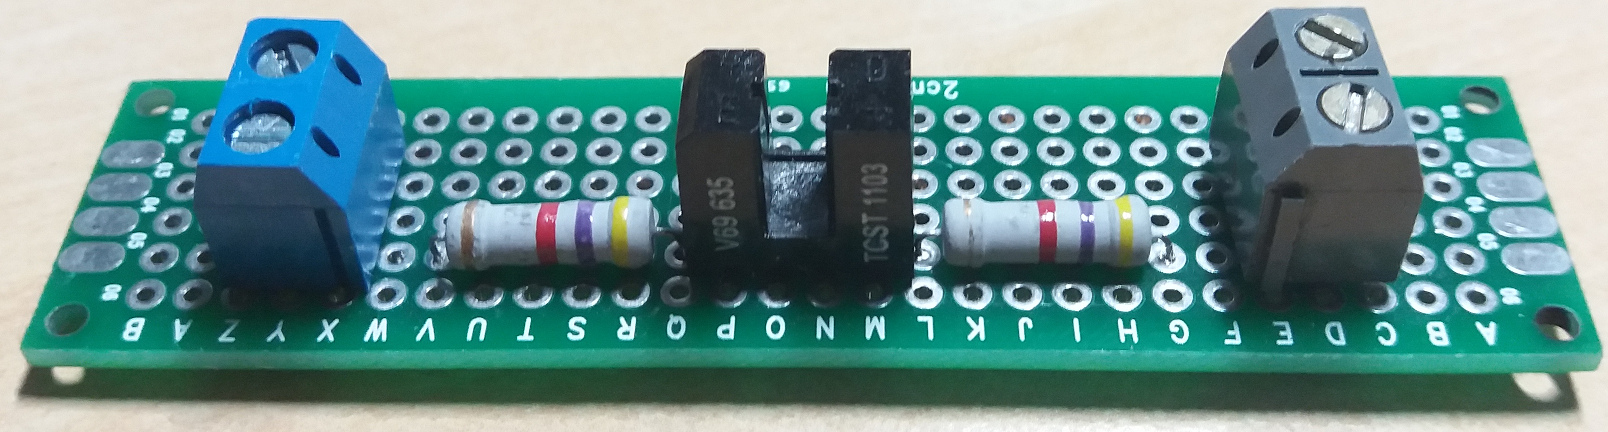
\includegraphics[width=0.6\textwidth]{czujnik_bazowania_PCB}
    \caption{Zdjęcie płytki PCB z zamontowanym układem z \cref{fig:uklad_transoptora}.}
    \label{fig:czujnik_bazowania_PCB}
\end{figure}

Płytka z czujnikiem bazowania została przytwierdzona do układu kulki i belki poniżej silnika. Sztywny, lekki i nieprzezroczysty element (chorągiewka) przyczepiony został na końcu korby tak, aby przechodził przez szczelinę enkodera w momencie skierowania korby pionowo w dół. Doświadczalnie ustalono, że w chwili zasłonięcia szczeliny (przy ruchu zgodnie ze wskazówkami zegara) licznik enkodera powinien otrzymać wartość \num{149}; wówczas pionowemu położeniu korby odpowiada wartość \num{0}.

%%%%%%%%
\section{Systemy napięć}
\label{sec:ch3_systemy_napiec}

Jak można zauważyć, elementy elektroniczne i elektromechaniczne użyte do zbudowania obiektu sterowania korzystają z poziomów logicznych o różnych napięciach (tabela \ref{tab:poziomy_napiec}). Wynika to z faktu połączenia obiektu typowo przemysłowego, jakim jest sterownik PLC Siemens S7-1211C, który wykorzystuje napięcie \SI{24}{\volt}, oraz elektroniki hobbystycznej (czujniki odległości, mostek H, enkoder), która wykorzystuje napięcia \SI{5}{\volt}. Dodatkowym utrudnieniem jest element wykonawczy, tj. silnik prądu stałego, o napięciu znamionowym 12V.

\begin{table}[h]
    \centering
    \begin{threeparttable}
        \caption{Podział modułów elektronicznych ze względu na wykorzystywany poziom napięcia.}
        \label{tab:poziomy_napiec}
        
        \begin{tabularx}{0.6\textwidth}{l | l}
            \toprule
            Element & Napięcie \\
            \midrule
            Sterownik PLC & \SI{24}{\volt} \\
            Płytka sygnałowa & \SI{5}{\volt} \\
            Mostek H (logika) & \SI{5}{\volt} \\
            Mostek H (zasilanie silnika)\tnote{a} & \SI{12}{\volt} \\
            Enkoder & \SI{5}{\volt} \\
            Czujniki odległości (zasilanie) & \SI{5}{\volt} \\
            Czujniki odległości (wyjście analogowe) & \SIrange{0,25}{3,1}{\volt} \\
            Sterownik PLC (wejścia analogowe) & \SIrange{0}{10}{\volt} \\
            Czujnik bazowania & \SI{24}{\volt} \\
            Przyciski & \SI{24}{\volt} \\
            Lampka sygnalizacyjna & \SI{24}{\volt} \\
            \bottomrule
        \end{tabularx}
        
        \begin{tablenotes}
            \footnotesize
            \item[a] wartość napięcia znamionowego silnika, zob. tab. \ref{tab:parametry_silnika}.
        \end{tablenotes}
    \end{threeparttable}
\end{table}

Obecność trzech systemów napięcia poskutkowała użyciem trzech oddzielnych zasilaczy: \SI{24}{\volt} o~mocy \SI{60}{\watt}, \SI{12}{\volt} o~mocy \SI{15}{\watt}, \SI{5}{\volt} o~mocy \SI{12,5}{\watt}. Wszystkie zasilacze zostały połączone wspólną masą.

%%%%%%%%
\section{Okablowanie i zabezpieczenia}
\label{sec:ch3_okablowanie_zabezpieczenia}

Połączenia elektryczne pomiędzy komponentami pracy zrealizowano za pomocą przewodów o przekroju \SI{0,75}{\milli\meter\squared}. Za wyjątkiem złącza silnika i enkodera, wszystkie przewody zakończone są zaciskanymi tulejami, co jest konieczne z powodu zastosowania złącz śrubowych.

Zasilanie po stronie \SI{230}{\volt} AC, \SI{50}{\hertz} zostało zabezpieczone instalacyjnym wyłącznikiem nadprądowym klasy B10.

Wyłącznik nadprądowy, zasilacz \SI{12}{\volt}, zasilacz \SI{24}{\volt} oraz sterownik PLC zostały przymocowane do wspólnej szyny DIN (TH \num{35}). Zasilacz impulsowy \SI{5}{\volt} nie był przeznaczony do montowania na szynie DIN (posiadał jednofazową wtyczkę elektryczną), dlatego na szynie DIN wspólnie ze sterownikiem i~pozostałymi zasilaczami zamontowano gniazdko elektryczne (połączone szeregowo za wyłącznikiem nadprądowym), do którego zasilacz \SI{5}{\volt} został podłączony.

Na drugiej szynie DIN zostały zamontowane cztery listwy przyłączeniowe przeznaczone dla każdego poziomu napięcia (zob. rozdział \ref{sec:ch3_systemy_napiec}): dwie dla napięcia \SI{0}{\volt} (wspólna masa), po jednej dla napięć \SI{5}{\volt}~oraz \SI{24}{\volt}. Z napięcia \SI{12}{\volt} korzysta tylko silnik, więc to połączenie zostało zrealizowane bezpośrednio, bez użycia listwy przyłączeniowej.

Użyte zasilacze posiadają drugą klasę ochronności, dlatego nie zostały dodatkowo podłączone przewodem ochronnym.

% TODO: dodaj zdjęcie szyn

%%%%%%%%
\section{Podsumowanie}

W niniejszym rozdziale przedstawiono układy elektryczne, elektroniczne i elektromechaniczne wykorzystane do stworzenia obiektu typu kulka i belka. Następnie umieszczono opisy poszczególnych elementów: sterownika PLC, płytki sygnałowej, silnika, enkodera, mostka~H i~czujników odległości. Przedstawiono charakterystyki czujników, sposób ich implementacji w sterowniku oraz sposób obliczania pozycji kulki. Następnie przedstawiono czujnik wykorzystywany do bazowania.

W kolejnych podrozdziałach poruszono kwestię różnych systemów napięć, zastosowanych zasilaczy, zabezpieczeń, okablowania i organizacji przewodów.

%---------------------------------------------------------------------------